\section{AOT translation overhead}
\label{sec-optimisations-aot-translation-overhead}
Now that we have good quality bytecode to work with, we can start addressing the overhead incurred during the AOT compilation process.

\subsection{Improving the peephole optimiser}
\label{sec-improved-peephole}
\begin{table}[hbt]
\centering
\caption{Improved peephole optimiser}
\label{tbl-improved-peephole}
\scriptsize
\addtolength{\tabcolsep}{-2pt}
\begin{tabular}{llll}
\toprule
JVM & AOT compiler & AVR & cycles \\
\hline
0: BRTARGET(0)   & \sccomment{record current addr} &                &   \\
1: SLOAD\_0      & emit\_LDD(R1,Y+0)        & LDD R1,Y+0     & 4 \\
                 & emit\_PUSH(R1)           & PUSH R1        & 4 \\
2: SCONST\_1     & emit\_LDI(R1,1)          & LDI R1,1       & 2 \\
                 & emit\_PUSH(R1)           & MOV R2,R1      & 1 \\
3: SUSHR         & emit\_POP(R2)            &                &   \\
                 & emit\_POP(R1)            & POP R1         & 4 \\
                 & emit\_RJMP(+2)           & RJMP +2        & 2 \\
                 & emit\_LSR(R1)            & LSR R1         & 2 \\
                 & emit\_DEC(R2)            & DEC R2         & 2 \\
                 & emit\_BRPL(-2)           & BRPL -2        & 3 \\
                 & emit\_PUSH(R1)           &                &   \\
4: SSTORE\_0     & emit\_POP(R1)            &                &   \\
                 & emit\_STD(Y+0,R1)        & STD Y+0,R1     & 4 \\
5: SLOAD\_0      & emit\_LDD(R1,Y+0)        & LDD R1,Y+0     & 4 \\
                 & emit\_PUSH(R1)           & MOV R2, R1     & 1 \\
6: SLOAD\_1      & emit\_LDD(R1,Y+2)        & LDD R1,Y+2     & 4 \\
                 & emit\_PUSH(R1)           &                &   \\
7: IF\_SCMPGT 0: & emit\_POP(R1)            &                &   \\
                 & emit\_POP(R2)            &                &   \\
                 & emit\_CP(R1,R2)          & CP R1,R2       & 2 \\
                 & emit\_branchtag(GT,0)    & BRGT 0:        & 2 (taken), \\
                 &                          &                & or 1 (not taken) \\
\bottomrule
\end{tabular}
\end{table}

Our first optimisation is a small but effective extension to the simple peephole optimiser. Instead of optimising only consecutive push/pop pairs, we can optimise any pair of push/pop instructions if the following holds for the instructions in between:
%\begin{itemize}
%   \item they contain the same number of \mycode{push} and \mycode{pop} instructions (the \mycode{pop} matches the \mycode{push})
%   \item they contain no branches
%   \item they may be do not use the \emph{target} register of the \mycode{pop}
%\end{itemize}

\begin{listing}
    \begin{minted}{asm}
    PUSH Rs
    ..
    ..       instructions in between: - contain the same number of push and pop instr.
    ..                                - contain no branches
    ..                                - do not use register Rd
    ..
    POP  Rd
     \end{minted}
\end{listing}

In this case the pair can be eliminated if Rs == Rd, otherwise it is replaced by a '\mycode{mov Rd, Rs}'. Two push/pop pairs remained in our earlier example Table \ref{tbl-basic-translation}. For the pair in instructions 5 and 7, the value is popped into register R2. Since instruction 6 does not use register R2, we can safely replace this pair with a direct move. In contrast, the pair in instructions 1 and 3 cannot be optimised since the value is popped into register R1, which is also used by instruction 2. The result is shown in Table \ref{tbl-improved-peephole}

% This optimisation adds 278 bytes to the optimiser, since it now needs to understand the bytecode well enough to determine which registers are being used.

\subsection{Simple stack caching}
\label{sec-optimisations-simple-stack-caching}
\begin{table}
\caption{Stack caching}
\label{tbl-simplestackcaching}
    \scriptsize\centerline{
    \begin{tabular}{llll|c|c|c|c} % NO SIMULATION DATA
    \toprule
                       &                                                      &                     &        & \multicolumn{4}{c}{cache state} \\
    Bytecode           & AOT compiler                                         & native code         & cycles & R1                   & R2                   & R3                   & R4                   \\
    \midrule
    \midrule
    0: BRTARGET(0)     & \sccomment{record current address}                   &                     &        & \sce{    }{   }{   } & \sce{    }{   }{   } & \sce{    }{   }{   } & \sce{    }{   }{   } \\
    1: SLOAD\_0        & operand\_1 = sc\_getfreereg()                        &                     &        & \sce{\use}{   }{   } & \sce{    }{   }{   } & \sce{    }{   }{   } & \sce{    }{   }{   } \\
                       & emit\_LDD(operand\_1,Y+0)                            & LDD R1,Y+0          &      4 & \sce{\use}{   }{   } & \sce{    }{   }{   } & \sce{    }{   }{   } & \sce{    }{   }{   } \\
                       & sc\_push(operand\_1)                                 &                     &        & \sce{Int1}{   }{   } & \sce{    }{   }{   } & \sce{    }{   }{   } & \sce{    }{   }{   } \\
    2: SCONST\_1       & operand\_1 = sc\_getfreereg()                        &                     &        & \sce{Int1}{   }{   } & \sce{\use}{   }{   } & \sce{    }{   }{   } & \sce{    }{   }{   } \\
                       & emit\_LDI(operand\_1,1)                              & LDI R2,1            &      2 & \sce{Int1}{   }{   } & \sce{\use}{   }{   } & \sce{    }{   }{   } & \sce{    }{   }{   } \\
                       & sc\_push(operand\_1)                                 &                     &        & \sce{Int2}{   }{   } & \sce{Int1}{   }{   } & \sce{    }{   }{   } & \sce{    }{   }{   } \\
    3: SUSHR           & operand\_1 = sc\_pop()                               &                     &        & \sce{Int1}{   }{   } & \sce{\use}{   }{   } & \sce{    }{   }{   } & \sce{    }{   }{   } \\
                       & operand\_2 = sc\_pop()                               &                     &        & \sce{\use}{   }{   } & \sce{\use}{   }{   } & \sce{    }{   }{   } & \sce{    }{   }{   } \\
                       & emit\_JMP(+2)                                        & JMP +2              &      2 & \sce{\use}{   }{   } & \sce{\use}{   }{   } & \sce{    }{   }{   } & \sce{    }{   }{   } \\
                       & emit\_LSR(operand\_2)                                & LSR R1              &      2 & \sce{\use}{   }{   } & \sce{\use}{   }{   } & \sce{    }{   }{   } & \sce{    }{   }{   } \\
                       & emit\_DEC(operand\_1)                                & DEC R2              &      1 & \sce{\use}{   }{   } & \sce{\use}{   }{   } & \sce{    }{   }{   } & \sce{    }{   }{   } \\
                       & emit\_BRPL(-2)                                       & BRPL -2             &      1 & \sce{\use}{   }{   } & \sce{\use}{   }{   } & \sce{    }{   }{   } & \sce{    }{   }{   } \\
                       & sc\_push(operand\_2)                                 &                     &        & \sce{Int1}{   }{   } & \sce{\use}{   }{   } & \sce{    }{   }{   } & \sce{    }{   }{   } \\
    4: SSTORE\_0       & operand\_1 = sc\_pop()                               &                     &        & \sce{\use}{   }{   } & \sce{    }{   }{   } & \sce{    }{   }{   } & \sce{    }{   }{   } \\
                       & emit\_STD(Y+0,operand\_1)                            & STD Y+0,R1          &      4 & \sce{\use}{   }{   } & \sce{    }{   }{   } & \sce{    }{   }{   } & \sce{    }{   }{   } \\
    5: SLOAD\_0        & operand\_1 = sc\_getfreereg()                        &                     &        & \sce{\use}{   }{   } & \sce{    }{   }{   } & \sce{    }{   }{   } & \sce{    }{   }{   } \\
                       & emit\_LDD(operand\_1,Y+0)                            & LDD R1,Y+0          &      4 & \sce{\use}{   }{   } & \sce{    }{   }{   } & \sce{    }{   }{   } & \sce{    }{   }{   } \\
                       & sc\_push(operand\_1)                                 &                     &        & \sce{Int1}{   }{   } & \sce{    }{   }{   } & \sce{    }{   }{   } & \sce{    }{   }{   } \\
    6: SLOAD\_1        & operand\_1 = sc\_getfreereg()                        &                     &        & \sce{Int1}{   }{   } & \sce{\use}{   }{   } & \sce{    }{   }{   } & \sce{    }{   }{   } \\
                       & emit\_LDD(operand\_1,Y+2)                            & LDD R2,Y+2          &      4 & \sce{Int1}{   }{   } & \sce{\use}{   }{   } & \sce{    }{   }{   } & \sce{    }{   }{   } \\
                       & sc\_push(operand\_1)                                 &                     &        & \sce{Int2}{   }{   } & \sce{Int1}{   }{   } & \sce{    }{   }{   } & \sce{    }{   }{   } \\
    7: IF\_SCMPGT(BT:0)& operand\_1 = sc\_pop()                               &                     &        & \sce{Int1}{   }{   } & \sce{\use}{   }{   } & \sce{    }{   }{   } & \sce{    }{   }{   } \\
                       & operand\_2 = sc\_pop()                               &                     &        & \sce{\use}{   }{   } & \sce{\use}{   }{   } & \sce{    }{   }{   } & \sce{    }{   }{   } \\
                       & emit\_CP(operand\_1, operand\_2);                    & CP R2,R1            &      2 & \sce{\use}{   }{   } & \sce{\use}{   }{   } & \sce{    }{   }{   } & \sce{    }{   }{   } \\
                       & emit\_branchtag(GT, 0);                              & BRGT 0:             &      2 & \sce{\use}{   }{   } & \sce{\use}{   }{   } & \sce{    }{   }{   } & \sce{    }{   }{   } \\
    \bottomrule
    \end{tabular}
    }
\end{table}



The improved peephole optimiser can remove part of the type 1 overhead, but still many cases remain where it cannot eliminate the push/pop instructions. We use a form of stack caching \cite{Ertl:1995dv} to eliminate most of the remaining push/pop overhead.

Stack caching is not a new technique. It was originally proposed for Forth interpreters in 1995. But the trade-offs involved are very different depending on the scenario it is applied in, and it turns out to be exceptionally well suited for a sensor node AOT compiler:

First, the VM in the original paper is an interpreter, which means the stack cache has to be very lightweight, or the overhead from managing it at run time will outweigh the time saved by reducing memory accesses. Since we only need to keep track of the cache state at translation time, this restriction does not apply for an AOT compiler and we can afford to spend more time managing it. Second, the simplicity of the approach means it requires very little memory: only 11 bytes of RAM and less than 1 KB of code more than the peephole optimiser.

The basic idea of stack caching is to keep the top elements of the stack in registers instead of main memory. We add a cache state to our VM to keep track of which registers are holding stack elements. For example, if the top two elements are kept in registers, an \mycode{ADD} instruction does not need to access main memory, but can simply add these registers, and update the cache state. Values are only spilled to memory when no more free registers are available.

In the baseline AOT approach, each bytecode instruction maps to a fixed sequence of native instructions that always use the same registers. Using stack caching, the registers are controlled by a stack cache manager that provides three functions:
\begin{itemize}
    \item \mycode{sc_getfree}: Instructions such as load instructions will need a free register to load the value into, which will later be pushed onto the stack. If all registers are in use, \mycode{sc_getfree} spills the register that's lowest on the stack to memory by emitting a \mycode{PUSH}, and then returns that register. Thus, the top of the stack is kept in registers, while lower elements may be spilled to memory.
    \item \mycode{sc_pop}: Pops the top element off the stack and tells the code generator in which register it can be found. If stack elements have previously been spilled to main memory and no  elements are left in registers, \mycode{sc_pop} will emit a real \mycode{POP} instruction to get the value back from memory.
    \item \mycode{sc_push}: Updates the cache state so the passed register is now at the top of the stack. This should be a register that was previously returned by \mycode{sc_getfree}, or \mycode{sc_pop}.
\end{itemize}

Using stack caching, code generation is split between the code generator, which emits the instructions that do the actual work, and the cache manager which manages the registers and may emit code to spill stack elements to memory, or to retrieve them again. But as long as enough registers are available, it will only manipulate the cache state.

In Table \ref{tbl-simplestackcaching} the same example is translated, this time using stack caching. The \mycode{emit_PUSH} and \mycode{emit_POP} instructions have been replaced by calls to the cache manager, and instructions that load something onto the stack start by asking the cache manager for a free register. The state of the stack cache is shown in the four columns added to the right. Currently it only tracks whether a register is on the stack or not. "Int1" marks the top element, followed by "Int2", etc. This example does not use the reference stack, but it is cached in the same way as the integer stack. A "*" marks a register that is marked as being used by the current instruction, but not currently on the stack. The next two optimisations will extend the cache state further.
 
The example only shows four registers, but the ATmega128 has 32 8-bit registers. Since CapeVM uses a 16-bit stack, they are managed as pairs. 10 registers are reserved, for example as a scratch register or to store a pointer to local variables, leaving 11 pairs available for stack caching.

\paragraph{Branches} Branch targets may be reached from multiple locations. We know the cache state if it was reached from the previous instruction, but not if it was reached through a branch. To ensure the cache state is the same on both paths, the whole stack is flushed to memory whenever we encounter either a branch or a \mycode{BRTARGET} instruction. 

This may seem bad for performance, but fortunately the stack is empty at almost all branches in the code generated by \mycode{javac}. A common exception is the ternary \mycode{? :} operator, which may cause a conditional branch with elements on the stack, but in most cases flushing at branches and branch targets does not result in any extra overhead.

\subsection{Popped value caching}
\label{sec-optimisations-popped-value-caching}
\begin{table*}[hbt]
\centering
\caption{Popped value caching}
\label{tbl-poppedvaluecaching}
\scriptsize
\addtolength{\tabcolsep}{-2pt}
\begin{tabular}{llll|c|c|c|c}
\toprule
JVM                & AOT compiler                                         & AVR                 & cycles & cache state R1       & cache state R2       & cache state R3       & cache state R4       \\
\hline
0: BRTARGET(0)     & \sccomment{record current address}                   &                     &        & \sce{    }{   }{   } & \sce{    }{   }{   } & \sce{    }{   }{   } & \sce{    }{   }{   } \\
1: SLOAD\_0        & operand\_1 = sc\_getfreereg()                        &                     &        & \sce{\use}{   }{   } & \sce{    }{   }{   } & \sce{    }{   }{   } & \sce{    }{   }{   } \\
                   & emit\_LDD(operand\_1,Y+0)                            & LDD R1,Y+0          & 4      & \sce{\use}{   }{   } & \sce{    }{   }{   } & \sce{    }{   }{   } & \sce{    }{   }{   } \\
                   & sc\_push(operand\_1)                                 &                     &        & \sce{Int1}{LS0}{   } & \sce{    }{   }{   } & \sce{    }{   }{   } & \sce{    }{   }{   } \\
2: SCONST\_1       & operand\_1 = sc\_getfreereg()                        &                     &        & \sce{Int1}{LS0}{   } & \sce{\use}{   }{   } & \sce{    }{   }{   } & \sce{    }{   }{   } \\
                   & emit\_LDI(operand\_1,1)                              & LDI R2,1            & 2      & \sce{Int1}{LS0}{   } & \sce{\use}{   }{   } & \sce{    }{   }{   } & \sce{    }{   }{   } \\
                   & sc\_push(operand\_1)                                 &                     &        & \sce{Int2}{LS0}{   } & \sce{Int1}{CS1}{   } & \sce{    }{   }{   } & \sce{    }{   }{   } \\
3: SUSHR           & operand\_1 = sc\_pop\_destructive()                  &                     &        & \sce{Int1}{LS0}{   } & \sce{\use}{   }{   } & \sce{    }{   }{   } & \sce{    }{   }{   } \\
                   & operand\_2 = sc\_pop\_destructive()                  &                     &        & \sce{\use}{   }{   } & \sce{\use}{   }{   } & \sce{    }{   }{   } & \sce{    }{   }{   } \\
                   & emit\_JMP(+2)                                        & JMP +2              & 2      & \sce{\use}{   }{   } & \sce{\use}{   }{   } & \sce{    }{   }{   } & \sce{    }{   }{   } \\
                   & emit\_LSR(operand\_2)                                & LSR R1              & 2      & \sce{\use}{   }{   } & \sce{\use}{   }{   } & \sce{    }{   }{   } & \sce{    }{   }{   } \\
                   & emit\_DEC(operand\_1)                                & DEC R2              & 1      & \sce{\use}{   }{   } & \sce{\use}{   }{   } & \sce{    }{   }{   } & \sce{    }{   }{   } \\
                   & emit\_BRPL(-2)                                       & BRPL -2             & 1      & \sce{\use}{   }{   } & \sce{\use}{   }{   } & \sce{    }{   }{   } & \sce{    }{   }{   } \\
                   & sc\_push(operand\_2)                                 &                     &        & \sce{\use}{   }{   } & \sce{Int1}{   }{   } & \sce{    }{   }{   } & \sce{    }{   }{   } \\
4: SSTORE\_0       & operand\_1 = sc\_pop\_tostore()                      &                     &        & \sce{    }{   }{   } & \sce{\use}{LS0}{   } & \sce{    }{   }{   } & \sce{    }{   }{   } \\
                   & emit\_STD(Y+0,operand\_1)                            & STD Y+0,R2          & 4      & \sce{    }{   }{   } & \sce{\use}{LS0}{   } & \sce{    }{   }{   } & \sce{    }{   }{   } \\
5: SLOAD\_0        & \sccomment{skip codegen, update cache state}         &                     &        & \sce{    }{   }{   } & \sce{Int1}{LS0}{   } & \sce{    }{   }{   } & \sce{    }{   }{   } \\
6: SLOAD\_1        & operand\_1 = sc\_getfreereg()                        &                     &        & \sce{\use}{   }{   } & \sce{Int1}{LS0}{   } & \sce{    }{   }{   } & \sce{    }{   }{   } \\
                   & emit\_LDD(operand\_1,Y+2)                            & LDD R1,Y+2          & 4      & \sce{\use}{   }{   } & \sce{Int1}{LS0}{   } & \sce{    }{   }{   } & \sce{    }{   }{   } \\
                   & sc\_push(operand\_1)                                 &                     &        & \sce{Int1}{LS1}{   } & \sce{Int2}{LS0}{   } & \sce{    }{   }{   } & \sce{    }{   }{   } \\
7: IF\_SCMPGT 0:   & operand\_1 = sc\_pop\_nondestructive()               &                     &        & \sce{\use}{LS1}{   } & \sce{Int1}{LS0}{   } & \sce{    }{   }{   } & \sce{    }{   }{   } \\
                   & operand\_2 = sc\_pop\_nondestructive()               &                     &        & \sce{\use}{LS1}{   } & \sce{\use}{LS0}{   } & \sce{    }{   }{   } & \sce{    }{   }{   } \\
                   & emit\_CP(operand\_1, operand\_2);                    & CP R1,R2            & 2      & \sce{\use}{LS1}{   } & \sce{\use}{LS0}{   } & \sce{    }{   }{   } & \sce{    }{   }{   } \\
                   & emit\_branchtag(GT, 0);                              & BRGT 0:             & 2      & \sce{\use}{LS1}{   } & \sce{\use}{LS0}{   } & \sce{    }{   }{   } & \sce{    }{   }{   } \\
\bottomrule
\end{tabular}
\addtolength{\tabcolsep}{2pt}
\end{table*}



Stack caching can eliminate most of the push/pop overhead, even when the stack depth increases. We now turn our attention to reducing the overhead resulting from load and store instructions.

A \emph{value tag} is added to each register's cache state to keep track of what value is currently held in the register, after it is popped from the stack. Some bytecode instructions have a value tag associated with them to indicate which value or variable they load, store, or modify. Each tag consist of a tuple (type, datatype, number). For example, the instructions \mycode{ILOAD_0} and \mycode{ISTORE_0}, which load and store the local integer variable with id 0, both have tag LI0, short for (local, int, 0). \mycode{SCONST_1} has tag CS1, or (constant, short, 1), etc. These tags are encoded as a 16-bit value.

The cache manager is extended with a \mycode{sc_can_skip} function. This function will examine the type of each instruction, its value tag, and the cache state. If it finds that the instruction loads a value that is already present in a register, it updates the cache state to put that register on the stack, and returns true to tell the main loop to skip code generation for this instruction.

Table \ref{tbl-poppedvaluecaching} shows popped value caching applied to our example. At first, the stack is empty. When \mycode{sc_push} is called, it detects the current instruction's value tag, and marks the fact that R1 now contains LS0. In \mycode{SUSHR}, the \mycode{sc_pop} has been changed to \mycode{sc_pop_destructive}. This tells the cache manager that the value in the register will be destroyed, so the value tag has to be cleared again since R1 will no longer contain LS0. The \mycode{SSTORE_0} instruction now calls \mycode{sc_pop_tostore} instead of  \mycode{sc_pop}, to inform the cache manager it will store this value in the variable identified by \mycode{SSTORE_0}'s value tag. This means the register once again contains LS0. If any other register was marked as containing LS0, the cache manager would clear that tag, since it is no longer accurate after we update the variable.

In bytecode instruction 5, we need to load LS0 again, but now the cache state shows that LS0 is already in R1. This means it does not need to load it from memory, but the cache manager can just update the cache state so that R1 is pushed onto the stack. At run time this \mycode{SLOAD_0} will have no cost at all.

There are a few more details to get right. For example if a value is loaded that's already on the stack, a move is emitted to copy it. When \mycode{sc_getfree} is called, it will try to return a register without a value tag. If none are available, the least recently used register is returned. This is done to maximise the chance we can reuse a value later, since recently used values are more likely to be used again.

\paragraph{Branches} As we do not know the state of the registers if an instruction is reached through a branch, we have to clear all value tags when we pass a \mycode{BRTARGET} instruction, meaning that any new loads will have to come from memory. At branches we can keep the value tags, because if the branch is not taken, the state of the registers in the next instruction is known.

\subsection{Mark loops}
\label{sec-optimisation-markloops}
\begin{table}
\caption{Mark loops}
\label{tbl-markloop}
    \begin{tabular}{llll|c|c|c|c}
    \toprule
    JVM                & AOT compiler                                         & AVR                 & cycles & cache state R1       & cache state R2       & cache state R3       & cache state R4       \\
    \midrule
    \midrule
    0: MARKLOOP(0,1)   & \sccomment{emit markloop prologue:}                  & LDD R1,Y+0          & 4      & \sce{    }{LS0}{PIN} & \sce{    }{   }{   } & \sce{    }{   }{   } & \sce{    }{   }{   } \\
                       & \sccomment{LS0 and LS1 are live}                     & LDD R2,Y+2          & 4      & \sce{    }{LS0}{PIN} & \sce{    }{LS1}{PIN} & \sce{    }{   }{   } & \sce{    }{   }{   } \\
    1: BRTARGET(0)     & \sccomment{record current address}                   &                     &        & \sce{    }{LS0}{PIN} & \sce{    }{LS1}{PIN} & \sce{    }{   }{   } & \sce{    }{   }{   } \\
    2: SLOAD\_0        & \sccomment{skip codegen, update cache state}         &                     &        & \sce{Int1}{LS0}{PIN} & \sce{    }{LS1}{PIN} & \sce{    }{   }{   } & \sce{    }{   }{   } \\
    3: SCONST\_1       & operand\_1 = sc\_getfreereg()                        &                     &        & \sce{Int1}{LS0}{PIN} & \sce{    }{LS1}{PIN} & \sce{\use}{   }{   } & \sce{    }{   }{   } \\
                       & emit\_LDI(operand\_1,1)                              & LDI R3,1            & 2      & \sce{Int1}{LS0}{PIN} & \sce{    }{LS1}{PIN} & \sce{\use}{   }{   } & \sce{    }{   }{   } \\
                       & sc\_push(operand\_1)                                 &                     &        & \sce{Int2}{LS0}{PIN} & \sce{    }{LS1}{PIN} & \sce{Int1}{CS1}{   } & \sce{    }{   }{   } \\
    4: SUSHR           & operand\_1 = sc\_pop\_destructive()                  &                     &        & \sce{Int1}{LS0}{PIN} & \sce{    }{LS1}{PIN} & \sce{\use}{   }{   } & \sce{    }{   }{   } \\
                       & operand\_2 = sc\_pop\_destructive()                  & MOV R4,R1           & 1      & \sce{    }{LS0}{PIN} & \sce{    }{LS1}{PIN} & \sce{\use}{   }{   } & \sce{\use}{   }{   } \\
                       & emit\_JMP(+2)                                        & JMP +2              & 2      & \sce{    }{LS0}{PIN} & \sce{    }{LS1}{PIN} & \sce{\use}{   }{   } & \sce{\use}{   }{   } \\
                       & emit\_LSR(operand\_2)                                & LSR R4              & 2      & \sce{    }{LS0}{PIN} & \sce{    }{LS1}{PIN} & \sce{\use}{   }{   } & \sce{\use}{   }{   } \\
                       & emit\_DEC(operand\_1)                                & DEC R3              & 1      & \sce{    }{LS0}{PIN} & \sce{    }{LS1}{PIN} & \sce{\use}{   }{   } & \sce{\use}{   }{   } \\
                       & emit\_BRPL(-2)                                       & BRPL -2             & 1      & \sce{    }{LS0}{PIN} & \sce{    }{LS1}{PIN} & \sce{\use}{   }{   } & \sce{\use}{   }{   } \\
                       & sc\_push(operand\_2)                                 &                     &        & \sce{    }{LS0}{PIN} & \sce{    }{LS1}{PIN} & \sce{\use}{   }{   } & \sce{Int1}{   }{   } \\
    5: SSTORE\_0       & \sccomment{emit MOV, update cache state}             & MOV R1,R4           & 1      & \sce{    }{LS0}{PIN} & \sce{    }{LS1}{PIN} & \sce{    }{   }{   } & \sce{    }{   }{   } \\
    6: SLOAD\_0        & \sccomment{skip codegen, update cache state}         &                     &        & \sce{Int1}{LS0}{PIN} & \sce{    }{LS1}{PIN} & \sce{    }{   }{   } & \sce{    }{   }{   } \\
    7: SLOAD\_1        & \sccomment{skip codegen, update cache state}         &                     &        & \sce{Int2}{LS0}{PIN} & \sce{Int1}{LS1}{PIN} & \sce{    }{   }{   } & \sce{    }{   }{   } \\
    8: IF\_SCMPGT(BT:0)& operand\_1 = sc\_pop\_nondestructive()               &                     &        & \sce{Int1}{LS0}{PIN} & \sce{    }{LS1}{PIN} & \sce{    }{   }{   } & \sce{    }{   }{   } \\
                       & operand\_2 = sc\_pop\_nondestructive()               &                     &        & \sce{    }{LS0}{PIN} & \sce{    }{LS1}{PIN} & \sce{    }{   }{   } & \sce{    }{   }{   } \\
                       & emit\_CP(operand\_1, operand\_2);                    & CP R2,R1            & 2      & \sce{    }{LS0}{PIN} & \sce{    }{LS1}{PIN} & \sce{    }{   }{   } & \sce{    }{   }{   } \\
                       & emit\_branchtag(GT, 0);                              & BRGT 1:             & 2      & \sce{    }{LS0}{PIN} & \sce{    }{LS1}{PIN} & \sce{    }{   }{   } & \sce{    }{   }{   } \\
    9: MARKLOOP(end)   & \sccomment{emit markloop epilogue: LS0 is live}      & STD Y+0,R1          & 4      & \sce{    }{LS0}{   } & \sce{    }{LS1}{   } & \sce{    }{   }{   } & \sce{    }{   }{   } \\
    \bottomrule
    \end{tabular}
\end{table}



Popped value caching reduces the type 2 overhead significantly, but the fact that we have to clear the value tags at branch targets means that a large part of this overhead still remains. This is particularly true for loops, since each iteration often uses the same variables, but the branch to start the next iteration clears those values from the stack cache. This is addressed by the next optimisation.

Again, we modify the infuser to add a new instruction to the bytecode: \mycode{MARKLOOP}. This instruction is used to mark the beginning and end of each innermost loop. \mycode{MARKLOOP} has a larger payload than most bytecode instructions: it contains a list of value tags that will appear in the loop and how often each tag appears, sorted in descending order.

When we encounter the \mycode{MARKLOOP} instruction, the VM may decide to reserve a number of registers and pin the most frequently used local variables to them. If it does, code is generated to prefetch these variables from memory and store them in registers. While in the loop, loading or storing these pinned variables does not require memory access, but only a manipulation of the cache state and possibly a simple move between registers. However, these registers will no longer be available for normal stack caching. Since 4 register pairs need to be reserved for code generation, at most 7 of the 11 available pairs can be used by mark loops.

Because the only way to enter and leave the loop is through the \mycode{MARKLOOP} instructions, the values can remain pinned for the whole duration of the block, regardless of the branches made inside. This lets us eliminate more load instructions, and also replace store instructions by a much cheaper move to the pinned register. \mycode{INC} instructions, which increment a local variable, operate directly on the pinned register, saving both a load and a store. All these cases are handled in \mycode{sc_can_skip}, bypassing the normal code generation. A small change to \mycode{sc_pop_destructive} is also necessary. If the register that is about to be popped is pinned, it cannot be used directly since this would corrupt the value of the pinned local variable. Instead, first a move to a free, non-pinned register, is emitted.

In Table \ref{tbl-markloop} the first instruction is now \mycode{MARKLOOP}, which tells the compiler local short variables 0 and 1 will be used. The compiler decides to pin them both to registers 1 and 2. The \mycode{MARKLOOP} instruction also tells the VM whether or not the variables are live, which they are at this point, so the two necessary loads are generated. This is reflected in the cache state. No elements are on the stack yet, but register 1 is pinned to LS0, and register 2 to LS1.

Next, LS0 is loaded. Since it is pinned to register 1, no code is generated, but the cache state is updated to reflect LS0 is now on top of the stack. After loading the constant 1, \mycode{SUSHR} pops both operands destructively. We cannot simply return register 1 since that would corrupt the value of variable LS0, so the second \mycode{sc_pop_destructive} emits a move to a free register and returns that register instead. Since LS0 is pinned, \mycode{SSTORE_0} can also be skipped, but \mycode{sc_can_skip} does need to emit a move back to the pinned register.

The next two loads are straightforward and can be skipped, and in the branch instruction the registers are popped non-destructively, so the pinned registers can be used directly.

Finally, the loop ends with another \mycode{MARKLOOP}, telling the compiler only local 0 is live at this point. This means LS0 in register 1 needs to be stored back to memory, but LS1 can be skipped since it is no longer needed.

\subsection{Instruction set modifications}
Next, we introduce five optimisations that target the type 3 overhead: cases where limitations in the JVM instruction set means some operations cannot be expressed as efficiently as in native code. This type of overhead is the most difficult to address because many of the transformations a desktop VM can do to avoid it take more resources than we can afford on a tiny device. Also, this type of overhead covers many different cases, and optimisations that help in a specific case may not be general enough to justify spending additional resources on it.

Still, there are a few things we can do by modifying the instruction set, that come at little cost to the VM and can make a significant difference.

Darjeeling's original instruction set is already quite different from the normal JVM instruction set. The most important change is the introduction of 16-bit operations. The JVM is internally a 32-bit machine, meaning \mycode{short}, \mycode{byte}, and \mycode{char} are internally stored as 32-bit integers. On a sensor device where memory is the most scarce resource, we often want to use shorter data types. To support this, Darjeeling internally stores values in 16-bit slots, and introduces 16-bit versions of all integer operations. For example, to multiply two shorts and store the result in a short, the 32-bit \mycode{IMUL} instruction is replaced by the 16-bit \mycode{SMUL} instruction. These transformations are all done by the infuser (see Figure \ref{fig-translation-process}).

However, the changes made by Darjeeling are primarily aimed at reducing memory consumption, not at improving performance. The infuser was extended to make several other changes. The \mycode{BRTARGET} and \mycode{MARKLOOP} instructions have already been discussed, and the \mycode{INVOKELIGHT} instruction is the topic of the next section. In addition to these, the following five other modifications were made to Darjeeling's instruction set:

\subsubsection{Constant bit shifts}
\label{sec-opt-constant-shift}
\begin{table*}[hbt]
\centering
\caption{Constant bit shift optimisation}
\label{tbl-constshift}
\scriptsize
\addtolength{\tabcolsep}{-2pt}
\begin{tabular}{llll|c|c|c|c}
\toprule
JVM                & AOT compiler                                         & AVR                 & cycles & cache state R1       & cache state R2       & cache state R3       & cache state R4       \\
\hline
0: MARKLOOP(0,1)   & \sccomment{emit markloop prologue:}                  & LDD R1,Y+0          & 4      & \sce{    }{LS0}{PIN} & \sce{    }{   }{   } & \sce{    }{   }{   } & \sce{    }{   }{   } \\
                   & \sccomment{LS0 and LS1 are live}                     & LDD R2,Y+2          & 4      & \sce{    }{LS0}{PIN} & \sce{    }{LS1}{PIN} & \sce{    }{   }{   } & \sce{    }{   }{   } \\
1: BRTARGET(0)     & \sccomment{record current address}                   &                     &        & \sce{    }{LS0}{PIN} & \sce{    }{LS1}{PIN} & \sce{    }{   }{   } & \sce{    }{   }{   } \\
2: SLOAD\_0        & \sccomment{skip codegen, just update cache state}    &                     &        & \sce{Int1}{LS0}{PIN} & \sce{    }{LS1}{PIN} & \sce{    }{   }{   } & \sce{    }{   }{   } \\
3: SUSHR\_CONST(1) & \sccomment{operand\_1 = sc\_pop\_destructive()}      & MOV R3,R1           & 1      & \sce{    }{LS0}{PIN} & \sce{    }{LS1}{PIN} & \sce{\use}{   }{   } & \sce{    }{   }{   } \\
                   & \sccomment{it\_LSR(operand\_1)}                      & LSR R3              & 2      & \sce{    }{LS0}{PIN} & \sce{    }{LS1}{PIN} & \sce{\use}{   }{   } & \sce{    }{   }{   } \\
                   & \sccomment{\_push(operand\_1)}                       &                     &        & \sce{    }{LS0}{PIN} & \sce{    }{LS1}{PIN} & \sce{Int1}{   }{   } & \sce{    }{   }{   } \\
4: SSTORE\_0       & \sccomment{emit MOV, update cache state}             & MOV R1,R3           & 1      & \sce{    }{LS0}{PIN} & \sce{    }{LS1}{PIN} & \sce{    }{   }{   } & \sce{    }{   }{   } \\
5: SLOAD\_0        & \sccomment{skip codegen, just update cache state}    &                     &        & \sce{Int1}{LS0}{PIN} & \sce{    }{LS1}{PIN} & \sce{    }{   }{   } & \sce{    }{   }{   } \\
6: SLOAD\_1        & \sccomment{skip codegen, just update cache state}    &                     &        & \sce{Int2}{LS0}{PIN} & \sce{Int1}{LS1}{PIN} & \sce{    }{   }{   } & \sce{    }{   }{   } \\
7: IF\_SCMPGT(BT:0)& operand\_1 = sc\_pop\_nondestructive()               &                     &        & \sce{Int1}{LS0}{PIN} & \sce{    }{LS1}{PIN} & \sce{    }{   }{   } & \sce{    }{   }{   } \\
                   & operand\_2 = sc\_pop\_nondestructive()               &                     &        & \sce{    }{LS0}{PIN} & \sce{    }{LS1}{PIN} & \sce{    }{   }{   } & \sce{    }{   }{   } \\
                   & emit\_CP(operand\_1, operand\_2);                    & CP R2,R1            & 2      & \sce{    }{LS0}{PIN} & \sce{    }{LS1}{PIN} & \sce{    }{   }{   } & \sce{    }{   }{   } \\
                   & emit\_branchtag(GT, 0);                              & BRGT 1:             & 2      & \sce{    }{LS0}{PIN} & \sce{    }{LS1}{PIN} & \sce{    }{   }{   } & \sce{    }{   }{   } \\
8: MARKLOOP(end)   & \sccomment{emit markloop epilogue: LS0 is live}      & STD Y+0,R1          & 4      & \sce{    }{LS0}{   } & \sce{    }{LS1}{   } & \sce{    }{   }{   } & \sce{    }{   }{   } \\
\bottomrule
\end{tabular}
\addtolength{\tabcolsep}{2pt}
\end{table*}



Most benchmarks described in Section \ref{sec-evaluation} do bit shifts by a constant number of bits. These appear not only in computation intensive benchmarks, but also as optimised multiplications or divisions by a power of 2, which are common in many programmes.

In JVM bytecode the shift operators take two operands from the stack: the value to shift, and the number of bits to shift by. While this is generic, it is not efficient for constant shifts: the constant first needs to be pushed onto the stack, and the bit shift is implemented as a simple loop which shifts one bit at a time. If the number of bits to shift by is already known, much more efficient code can be generated.

Note that this is different from other arithmetic operations with a constant operand. For operations such as addition, the translation process results in loading the constant and performing the addition, which is similar to what \mycode{avr-gcc} generates in most cases. An addition takes just as long when the operand is taken from the stack, as when it is a constant. 

The mismatch is in the fact that while the JVM instruction set is more general, with both operands being variable for both bit shifts and other arithmetic operations, the native instruction set can only shift by a single bit. This means that to shift by a number of bits that is unknown until run time, a loop must be generated to shift one bit at a time, which is much slower than the code that can be generated for a shift by a constant number of bits.

We optimise these cases by adding \mycode{_CONST} versions of the bit shift instructions \mycode{ISHL}, \mycode{ISHR}, \mycode{IUSHR}, \mycode{SSHL}, \mycode{SSHR}, and \mycode{SUSHR}. We add a simple scan to the infuser to find constant loads that are immediately followed by a bit shift. For these cases the constant load is removed, and the bit shift instruction, for example \mycode{ISHL}, is replaced by \mycode{ISHL_CONST}, which has a one byte constant operand in the bytecode containing the number of bits to shift by. On the VM side, implementing these six \mycode{_CONST} versions of the bit shift opcodes adds 444 bytes to the VM, but it improves performance, sometimes very significantly, for all but three of the benchmarks.

Surprisingly, after this was implemented, one benchmark performed better than native C. We found that \mycode{avr-gcc} does not optimise constant shifts in all cases. Since the goal is to examine how close a sensor node VM can come to native performance, it would be unfair to include an optimisation that is not found in the native compiler, but could easily be added. We implemented a version that is close to what \mycode{avr-gcc} does, but never better. The VM only considers cases that are optimised by \mycode{avr-gcc}. For these, first whole byte moves are emitted if the number of bits to shift by is 8 or more, followed by single bit shifts for the remainder.

The result when applied to our example is shown in Table \ref{tbl-constshift}, where the \mycode{SCONST_1} and \mycode{SUSHR} instructions have been replaced by a single \mycode{SUSHR_CONST} instruction. The total cost is now 20 cycles, but 12 of these are spent before and after the loop, while each iteration now only takes 8 cycles, a significant improvement from the 48 cycles spent in the original version in Table \ref{tbl-basic-translation}.


\subsubsection{\mycode{GET/PUTFIELD_A_FIXED} reference field access}
The \mycode{GETFIELD_*} and \mycode{PUTFIELD_*} instructions are used to access fields in objects. Because references and integer slots are split, the offset from the object pointer is known at compile time only for integer fields, but not for reference fields. As shown in Figure \ref{fig-super-class-sub-class-field-layout}, integer fields will be at the same offset, regardless of whether an object is of the compile-time type, or a subclass. References fields may shift up in subclasses, so \mycode{GETFIELD_A} and \mycode{PUTFIELD_A} must examine the object's type at run time and calculate the offset accordingly, adding significant overhead.

\begin{figure}
\centering
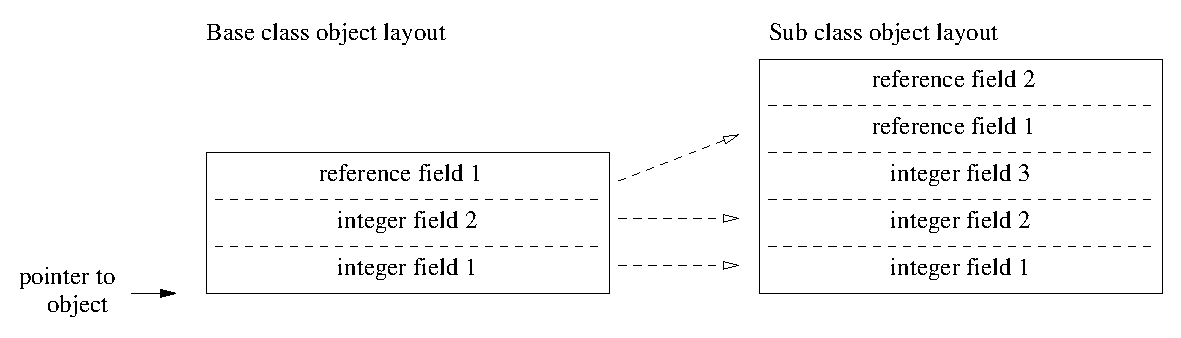
\includegraphics[width=0.7\linewidth]{super-class-sub-class-field-layout.eps}
\caption{Base class and sub class layout}
\label{fig-super-class-sub-class-field-layout}
\end{figure}

This overhead can be avoided if we can be sure of the offset at compile time, which is the case if the compile-time type is marked \mycode{final}. In this case the infuser will replace the \mycode{GETFIELD_A} or \mycode{PUTFIELD_A} opcode with a \mycode{_FIXED} version so the VM knows it is safe to determine the offset at translation time. Conveniently, one of the optimisations ProGuard does, is to mark any class that is not subclassed as \mycode{final}, so most of this is automatic.

\paragraph{Alternative solutions} An alternative we considered is to let go of the split for references and integers for object fields and mix them, so the offsets for reference fields would also be known at compile time. To allow the garbage collector to find the reference fields we could either extend the class descriptors with a bit map indicating the type of each slot, or let the garbage collector scan all classes in the inheritance line of an object.

We chose our solution because it is easier to implement and adds only a few bytes to the VM size, while the garbage collector is already one of the most complex components of the VM. Also, we found that almost all classes in our benchmarks could be marked \mycode{final}. Either solution would work, and the alternative could be considered as a more general solution.

\paragraph{Evaluation}
The impact of this optimisation is significant, but we decided not to include it in our evaluation since the overhead is the result of implementation choices in Darjeeling, which was optimised for size rather than performance. This means the overhead is a result of a Darjeeling specific choice, rather than a direct result of the AOT techniques or the JVM's design. Therefore, all results reported in this paper are with this optimisation already enabled.

Since the split architecture has many advantages in terms of complexity and VM size, we still feel it is important to mention this as an example of the kind of trade-offs faced when optimising for performance.

\subsubsection{\mycode{SIMUL} 16-bit to 32-bit multiplication}
While Darjeeling already introduced 16-bit arithmetic operations, it does not cover the case of multiplying two 16-bit shorts, and storing the result in a 32-bit integer. In this case the infuser would emit \mycode{S2I} instructions to convert the operands to two 32-bit integers, and then use the normal \mycode{IMUL} instruction for full 32-bit multiplication. On an 8-bit device, this is significantly more expensive than 16x16 to 32-bit multiplication.

We added a new opcode, \mycode{SIMUL}, for this case, which the infuser will emit if it can determine the operands are 16-bit, but the result is used as a 32-bit integer.

We could add more instructions, for example, \mycode{SIADD} for 16-bit to 32-bit addition, \mycode{BSMUL} for 8-bit to 16-bit multiplication, etc. But there is a trade-off between the added complexity of an optimisation and the performance improvement it yields, and for these cases this is much smaller than for \mycode{SIMUL}.

\subsubsection{16-bit array indexes}
The normal JVM array access instructions (\mycode{IASTORE}, \mycode{IALOAD}, etc) use a 32-bit index. On a sensor node with only a few KB of memory, we will never have arrays that require such large indexes, so we modified the array access instructions to use a 16-bit index instead. 

This complements one of the manual optimisations discussed in Section \ref{sec-optimisations-manual-java-source-optimisation}. Using short values as index variables makes operations on the index variable cheaper, while changing the operand of the array access instructions reduces the amount of work the array access instruction needs to do and the number of registers it requires.

In CapeVM's bytecode, the array access instructions are named \mycode{GETARRAY} and \mycode{PUTARRAY} to be in line with \mycode{GET/PUTFIELD} and \mycode{GET/PUTSTATIC}.

\subsubsection{Support for constant arrays}
\label{sec-opt-constant-arrays}
Finally, while Java allows us to declare variables as \mycode{final}, this is only a language level feature, and the VM has no concept of constant data. This is not surprising, since most physical CPUs do not make the distinction either, but on a sensor node code and data memory are split. The amount of flash memory is usually several times larger than the available RAM, so constant data should be kept in flash instead of wasting precious RAM on data that never changes.

This is especially important for arrays of constant data, which are common in sensor node applications. For example, the \mybench{FFT} benchmark contains an array of precalculated sine wave values. When we implement this as a \mycode{final} Java array, the compiler emits a static class initialiser that creates a normal Java array object, and then uses the array access instructions to initialise each element individually, as shown in Listing \ref{lst-constant-array-initialisation}. The \mycode{final} keyword only affects the reference to the \mycode{Sinewave} array, but not the array itself.

\begin{listing}
\begin{minted}{java}
    private final static byte Sinewave[] = new byte[] {
        0, 3, 6, 9, 12, 15, 18, 21,
        ...
        -24, -21, -18, -15, -12, -9, -6, -3, 
    };
\end{minted}
\begin{minted}{c}
    sspush(256); newarray;                     // create the array
    adup; sconst_0;    sconst_0;   putarray_b;    // set index 0
    adup; sconst_1;    sconst_3;   putarray_b;    // set index 1
    adup; sconst_2;    bspush(6);  putarray_b;    // set index 2
    ...
    adup; bspush(255); bspush(-3); putarray_b;    // set index 255
\end{minted}
\caption{Array of constant data from the 8-bit FFT benchmark, and the resulting bytecode without the constant array optimisation}
\label{lst-constant-array-initialisation}
\end{listing}


There are two problems with this: (i) the array will occupy scarce RAM; and (ii) initialising array elements using bytecode instructions requires 4 instructions per element, resulting in 1663 bytes of bytecode to initialise a 256 byte array, which expands even further after AOT compilation.

To solve this, four new \mycode{GETCONSTARRAY} instructions are introduced to read from constant arrays of ints, shorts, chars or bytes. The normal \mycode{GETARRAY} instructions take two operands from the stack: the reference to the array, and the index of the element to load. The \mycode{GETCONSTARRAY} instructions only read the index from the stack, and have the id of an array in the constant pool encoded as a single byte operand in the bytecode instruction.

The infuser is modified to place constant arrays in the constant pool. Since the current infuser works on the \mycode{javac} output, it requires each constant array to be placed in a wrapper class with the \mycode{@ConstArray} annotation, which simplifies processing them considerably.

When the infuser loads a class and finds the \mycode{@ConstArray} annotation, it parses the \mycode{<clinit>} class initialiser to extract the data for the constant array. The class initialiser is then removed, and the data for the constant array is added to the constant pool.

When the infuser processes a method's bytecode, it analyses the operand stack. If a \mycode{GETSTATIC_A} instruction loads a reference to an array in a \mycode{@ConstArray} class onto the stack, the entry used for stack analysis is marked. This allows the infuser to the find the corresponding \mycode{GETARRAY} instruction that consumes this reference from the stack. The infuser then replaces it with a \mycode{GETCONSTARRAY} instruction, which carries the constant pool id of the array as a bytecode operand, and removes the original \mycode{GETSTATIC_A}.

This means the array no longer takes up any RAM, and only uses the amount of flash required to hold the data and a four byte header. Another advantage of this approach is that the reference no longer needs to be loaded onto the stack. This eliminates the \mycode{GETSTATIC_A} instruction, reduces the stack depth, and slightly simplifies the address calculation to find the correct offset since constant arrays do not have the small header used for normal arrays. This compensates for the fact that reading from flash is slightly more expensive at 3 cycles per byte, compared to 2 for reading from RAM. 

\paragraph{Alternative solutions}
A disadvantage of the chosen approach is that the constant arrays cannot be used for anything except directly reading from them. Since no array object is created, we cannot assign a reference to it to a variable, for example to decide at run time whether to read from one array or another.

This would be possible if we keep the \mycode{GETSTATIC_A} instruction, but use it to load a special reference to the constant array onto the stack instead. However, this would remove the advantages of not having to load the reference and result in a more complex design.

Since all examples found in the benchmarks directly read from the constant arrays, we choose the simpler option, and note that such a run time decision could also be implemented using an \mycode{if} statement or a small helper function, albeit at a higher cost. 
